\chapter{研究の準備}\label{cha:Preparation}

本章では、\tool{}を試作する際に必要となる前提知識を説明する。

\section{Python}\label{sec:Python}
Python \cite{python} は、Guido van Rossum が 1989 年から 1991 年にかけて開発した、インタプリタ型のプログラミング言語である。
現在では、機械学習やデータサイエンス、Web 開発など幅広い分野で用いられている。
本研究で試作する \tool は、Python を用いて実装する。
\tool を実装する際に使用する、3つのPython の標準ライブラリのモジュールを、以下に示す。

\begin{itemize}
    \item re \\
    reモジュールは、正規表現を用いるための機能を提供するモジュールである。文字列の検索、置換など、文字列操作の機能を提供する。
    本研究では、要求仕様情報リスト生成処理 (\ref{subsec:req_extraction}節で後述) およびテストケース情報リスト生成処理 (\ref{sec:testcase-data-extraction}節で後述) において、入力の要求仕様書とテストケースから要求仕様ID、テストケースIDを抽出する際に使用する。
    \item csv \\
    csv モジュールは、CSV (Comma Separated Values) 形式のファイルの読み込みや書き込みを行うための機能を提供するモジュールである。
    本研究では、要求仕様情報リスト生成処理およびテストケース情報リスト生成処理において、CSV形式の要求仕様書とテストケースを辞書型オブジェクトとして読み込むために、csv モジュールのDictReader関数を使用する。
    \item http.server \\
    http.server モジュールは、簡易的なHTTPサーバーを構築するための機能を提供するモジュールである。主に、開発や検証を目的として、静的ファイルの配信やHTTP通信の動作確認を容易に行うことができる。
    本研究では、TCVダイアグラム出力処理 (\cref{subsec:diagram-generation-process}節で後述)でSVG画像として保存したTCVダイアグラム(\cref{sec:testcase_visualization_diagram}で後述)をブラウザ上で表示するための、ローカルサーバーを起動する際に使用する。
\end{itemize}


\section{MeCab}\label{sec:Mecab}
MeCabは、京都大学情報学研究科 -- 日本電信電話株式会社コミュニケーション科学基礎研究所 共同研究ユニットプロジェクトを通じて開発された、
オープンソース形態素解析エンジンである\cite{mecab}。
MeCab を用いることで、日本語の文章の分かち書きや、単語の品詞を取得できる。
MeCab は C++ で記述されており、Python3 で利用するためのオープンソースのラッパーライブラリに、mecab-python3\cite{mecab_python3}がある。

本研究では、形態素解析処理(\cref{sec:morphological_analysis}節で後述)において、mecab-python3 から呼び出した MeCab を用いて、形態素解析を行う。
なお、本研究ではMeCabの形態素解析に用いる辞書として、IPA辞書\cite{mecab}を利用する。

\section{PlantUML}\label{sec:PlantUML}
PlantUML \cite{plantuml} は、テキストデータから UML のダイアグラムや UML 以外の様々なタイプのダイアグラムを生成できるツールである。
テキストデータは、PlantUML 独自の構文で記述する。以降、PlantUML の構文で書いたテキストデータを、PlantUML コードと呼ぶ。

本研究では、PlantUML コードからTCVダイアグラムを生成するために、PlantUMLのオープンソースのJavaライブラリ\cite{plantuml_lib}を使用する。

\section{Jaccard係数}\label{sec:Jaccard}
Jaccard係数は、2つの集合の類似度を測る指標の1つである。テキストに含まれる単語を集合の要素と見なすことで、テキスト間の類似度を算出できる。
集合$A$と$B$のJaccard係数$J(A,B)$を算出する式(\ref{eq:jaccard})を、以下に示す。
Jaccard係数は、$1$に近いほど2つのテキストは類似していることを示し、$0$に近いほど2つのテキストは類似していないことを示す。

\begin{equation}\label{eq:jaccard}
    J(A,B) = \frac{|A \cap B|}{|A \cup B|} \quad (0 \le J(A,B) \le 1)
\end{equation}

例として、テキスト$A$と$B$から得られた単語の集合を、それぞれ$A = \{x, y, z, w\}$、$B = \{x, y, v\}$とする。この場合、式(\ref{eq:jaccard})によって、類似度は以下のように算出できる。
\[J(A,B) = \frac{\{x, y\}}{\{x, y, z, w, v\}} = \frac{2}{5} = 0.4\]

本研究では、類似度算出処理(\ref{subsec:similarity_calculation}節で後述)において、要求仕様とテストケースのテキスト間の類似度を、Jaccard係数を用いて算出する。

\section{EARS}\label{sec:EARS}
EARS (Easy Approach to Requirements Syntax) は、Rolls-Royce社のMavinらによって提案された、自然言語で要求仕様を記述するための簡易構文テンプレートである\cite{ears}。
制約のない自然言語で記述する要求仕様には、曖昧性や複雑性、検証不能性などの問題が存在する場合がある。
EARSは、特定のテンプレートに沿って要求仕様を記述することによって、これらの問題を回避するアプローチである。

本研究では、EARSを参考に、以下を要求仕様テンプレートとして定義する。
\begin{center}
「\{前提条件\}場合、\{トリガー\}時、\{システム名\} は \{システム応答\}べきである」
\end{center}

\section{入力対象の要求仕様書}\label{sec:reqspec}
\tool は、以下の7つの条件をすべて満たす要求仕様書を入力対象とする。

\begin{itemize}
    \item 日本語で記述している。
    \item CSVファイル(.csv)として記述している。
    \item 機能要件を対象としている。
    \item 各要求仕様は、要求仕様記述項目(表\ref{tb:reqspec_item}参照)の定義に従って記述している。
    \item 「前提条件」および「システム応答」の項目は、2個以上の記述がある場合、読点(、)で区切って記述している。
    \item 各要求仕様に固有の要求仕様IDを割り当てている。
    \item 要求仕様IDは、要求仕様IDの命名規則に従っている。
\end{itemize}

\begin{table}[tp]
        \caption{要求仕様記述項目}\label{tb:reqspec_item}
        \centering
        \begin{tabular}{c|l|l}
            項目名 & \multicolumn{1}{c|}{定義} & \multicolumn{1}{c}{記述ルール} \\
            \hline
            \hline
            要求仕様ID & 要求仕様を一意に識別するためのID & 1個 (必須) \\
            \hline
            要求仕様名 & 要求仕様の概要を表す名称 & 1個 (必須) \\
            \hline
            前提条件 & システムが応答するために必要な状態や条件 & 0個以上 (任意) \\
            \hline
            トリガー & システムの動作を開始させる具体的なイベントや事象 & 0または1個 (任意) \\
            \hline
            システム応答 & システムが実行すべき動作や出力結果 & 1個以上 (必須) \\
            \hline
        \end{tabular}
    \end{table}

\tool の入力対象である要求仕様書の例を、図\ref{fig:reqspec_sample1}に示す。

\begin{figure}[tp]
        \centering
        \fbox{
            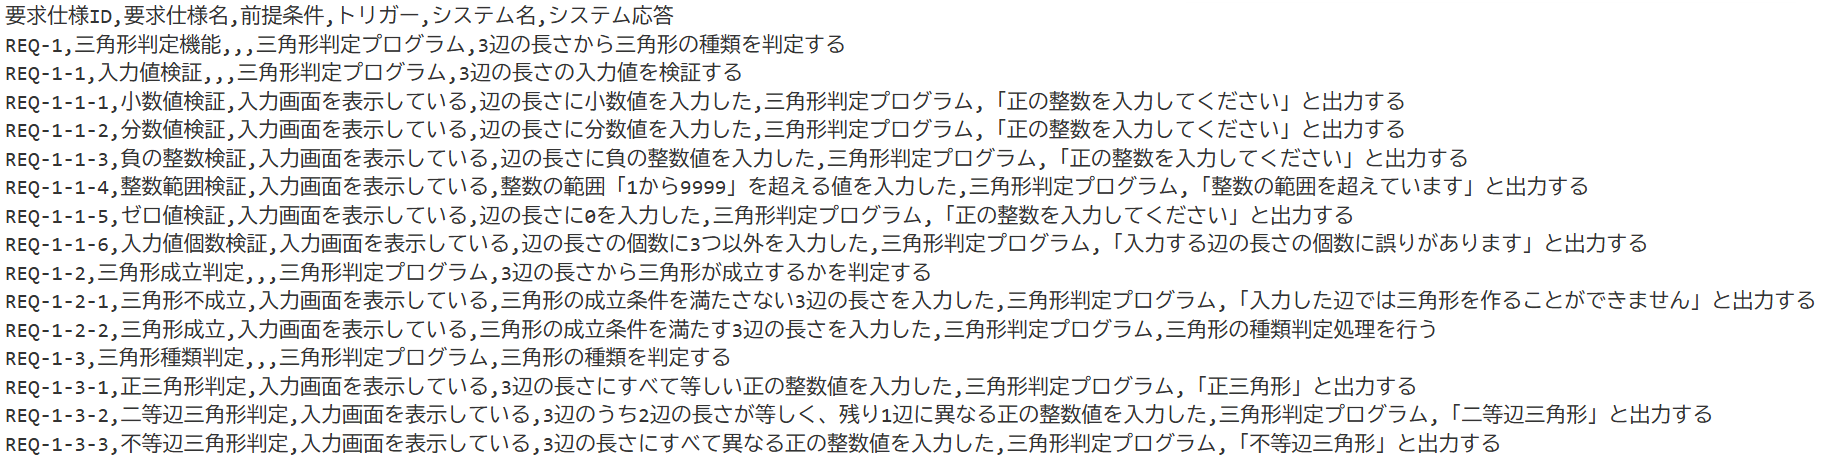
\includegraphics[width=0.96\textwidth]{images/reqspec_sample1.png}
            }
            \caption{\tool の入力対象である要求仕様書の例}
            \label{fig:reqspec_sample1}
        \end{figure}

\begin{description}
    \item[要求仕様記述項目]\mbox{}\\
    本研究では、各要求仕様に記述する項目を、要求仕様記述項目として定義する。
    表\ref{tb:reqspec_item}に、要求仕様記述項目を示す。
    要求仕様記述項目のうち、「前提条件」、「トリガー」、および「システム応答」の項目は、 \ref{sec:EARS}節で述べた要求仕様テンプレートの各要素に対応している。
    要求仕様記述項目は、5つの項目と項目ごとの記述ルールで定義する。
    なお、「トリガー」の項目は0または1個であるため、テキスト中に読点を含む場合でも1個のトリガーとして扱う。
    
    \item[要求仕様IDの命名規則]\mbox{}\\
    本研究では、要求仕様IDの命名規則は、Pythonの正規表現(\ref{sec:Python}節参照)を用いて、以下の形式で定義する。

    \begin{center}
        \textasciicircum{}REQ-[1-9][0-9]*(-[1-9][0-9]*)*\$
    \end{center}

    要求仕様IDは、ハイフン (\texttt{-}) で区切った番号により、要求仕様の親子関係を階層的に表現できる。
    例えば、REQ-1-2-3の場合、REQ-1が第1階層(親)、REQ-1-2が第2階層(子)、REQ-1-2-3が第3階層(孫)となる。
    この階層関係を用いて各要求仕様を記述することにより、抽象的な要求から具体的な要求へと分解して記述できる。

\end{description}

\section{入力対象のテストスイート}\label{sec:testcase}
\tool は、以下の7つの条件をすべて満たすテストスイートを入力対象とする。
なお、本研究では、テストスイートとは複数のテストケースの集合とする。

\begin{itemize}
    \item 日本語で記述している。
    \item CSVファイル(.csv)として記述している。
    \item ファイル名が、「テストスイート名.csv」である。
    \item 各テストケースは、テストケース記述項目(表\ref{tb:testcase_item}参照)の定義に従って記述している。
    \item 各テストケースは1つの要求仕様のみを検証対象とし、同一の要求仕様を検証するテストケースは複数存在しない。
    \item 入力対象とする、すべてのテストスイート間で重複しない固有なテストケースIDを、各テストケースに割り当てている。
    \item テストケースIDは、テストケースIDの命名規則に従っている。
\end{itemize}

\tool の入力対象であるテストスイートの例を、図\ref{fig:tc_2}に示す。

\begin{figure}[tp]
        \centering
        \fbox{
        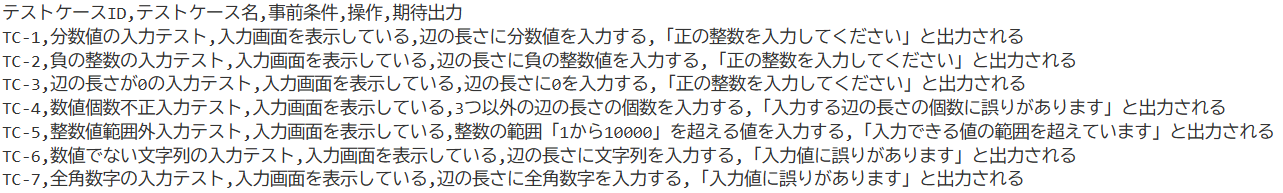
\includegraphics[width=0.96\textwidth]{images/tc_2.png}
        }
        \caption{\tool の入力対象であるテストスイートの例}
        \label{fig:tc_2}
    \end{figure}

\begin{table}[tp]
    \caption{テストケース記述項目}\label{tb:testcase_item}
    \centering
    \begin{tabular}{c|l|l}
        項目名 & \multicolumn{1}{c|}{定義} & \multicolumn{1}{c}{記述ルール} \\
        \hline
        \hline
        テストケースID & テストケースを一意に識別するためのID & 1個 (必須) \\
        \hline
        テストケース名 & テストケースの概要を表す名称 & 1個 (必須) \\
        \hline
        事前条件 & テストを実行する前に、システムが満たしているべき状態や環境 & 必須 \\
        \hline
        操作 & テスト実行時に行う具体的な操作 & 必須 \\
        \hline
        期待出力 & 操作の結果として想定されるシステムの出力 & 必須 \\
        \hline
    \end{tabular}
\end{table}

\begin{description}
    \item[テストケース記述項目]\mbox{}\\
    本研究では、各テストケースに記述する項目を、テストケース記述項目として定義する。
    表\ref{tb:testcase_item}に、テストケース記述項目を示す。
    テストケース記述項目は、表\ref{tb:testcase_item}に示す5つの項目と項目ごとの記述ルールで定義する。

    \item[テストケースIDの命名規則]\mbox{}\\
    本研究では、テストケースIDの命名規則は、Pythonの正規表現(\ref{sec:Python}節参照)を用いて、以下の形式で定義する。

    \begin{center}
        \textasciicircum{}TC-[1-9][0-9]*\$
    \end{center}

    テストケースIDは、要求仕様IDで定めた階層関係では表現せず、TC\texttt{-}から始まり、その後に一意の番号が続く形式とする。
\end{description}

\section{要求仕様とテストケースの対応関係に関する用語}\label{sec:words}
本研究で用いる、3つの要求仕様とテストケースの対応関係に関する用語を、以下に示す。

\begin{itemize}
    \item 対応関係\\
    特定のテストケースが、特定の要求仕様を検証する関係を、対応関係と呼ぶ。

    \item 対応付け要素\\
    要求仕様とテストケースの対応関係を抽出する際に用いる要素を、対応付け要素と呼ぶ。\\
    要求仕様とテストケースの対応付け要素を、表\ref{tb:traceability}に示す。
    本研究では、以下の3種類の対応付け要素間のテキストを比較することで、要求仕様とテストケースの対応関係を抽出する。

    \begin{itemize}
        \item 「前提条件」と「事前条件」
        \item 「トリガー」と「操作」
        \item 「システム応答」と「期待出力」
    \end{itemize}

    \begin{table}[tp]
        \caption{要求仕様とテストケースの対応付け要素}\label{tb:traceability}
        \centering
        \begin{tabular}{l|l|l}
            \multicolumn{1}{c|}{要求仕様の対応付け要素} & \multicolumn{1}{c|}{テストケースの対応付け要素} & \multicolumn{1}{c}{対応付けにおける役割} \\
            \hline
            \hline
            前提条件 & 事前条件 & システムの初期状態の一致を判定 \\
            \hline
            トリガー & 操作 & システムへの働きかけの一致を判定 \\
            \hline
            システム応答 & 期待出力 & システムの振る舞いの一致を判定 \\
            \hline
        \end{tabular}
    \end{table}

    \item 対応付け可能な要求仕様\\
    要求仕様の対応付け要素 (「前提条件」、「トリガー」、「システム応答」)の値が全て空文字列でない要求仕様を、対応付け可能な要求仕様と呼ぶ。\\
    要求仕様の対応付け要素のうち、いずれか$1$つでも対応付け要素の値が空文字列である要求仕様は、対応付け不可能な要求仕様と呼び、テストケースとの対応付けの対象外とする。

\end{itemize}
